%%%%%%%%%%%%%%%%%%%%%%%%%%%%%%%%%%%%%%%%%%%%%%
%% Compile: XeLaTeX BibTeX XeLaTeX XeLaTeX
%% Loesung-Handout: Antonio Machicao y Priemer
%% Course: GK Linguistik
%%%%%%%%%%%%%%%%%%%%%%%%%%%%%%%%%%%%%%%%%%%%%%

%\documentclass[a4paper,10pt, bibtotoc]{beamer}
\documentclass[10pt,handout]{beamer}

%%%%%%%%%%%%%%%%%%%%%%%%
%%     PACKAGES      
%%%%%%%%%%%%%%%%%%%%%%%%

%%%%%%%%%%%%%%%%%%%%%%%%
%%     PACKAGES       %%
%%%%%%%%%%%%%%%%%%%%%%%%



%\usepackage[utf8]{inputenc}
%\usepackage[vietnamese, english,ngerman]{babel}   % seems incompatible with german.sty
%\usepackage[T3,T1]{fontenc} breaks xelatex
\usepackage{lmodern}

\usepackage{amsmath}
\usepackage{amsfonts}
\usepackage{amssymb}
%% MnSymbol: Mathematische Klammern und Symbole (Inkompatibel mit ams-Packages!)
%% Bedeutungs- und Graphemklammern: $\lsem$ Tisch $\rsem$ $\langle TEXT \rangle$ $\llangle$ TEXT $\rrangle$ 
\usepackage{MnSymbol}
%% ulem: Strike out
\usepackage[normalem]{ulem}  

%% Special Spaces (s. Commands)
\usepackage{xspace}				
\usepackage{setspace}
%	\onehalfspacing

%% mdwlist: Special lists
\usepackage{mdwlist}	

\usepackage[noenc,safe]{tipa}

% maybe define \textipa to use \originalTeX to avoid problems with `"'.
%
%	\ex \textipa{\originalTeX [pa.pa."g\t{aI}]}

%

\usepackage{etex}		%For Forest bug

%
%\usepackage{jambox}
%


%\usepackage{forest-v105}
%\usepackage{modified-langsci-forest-setup}

\usepackage{xeCJK}
\setCJKmainfont{SimSun}


%\usepackage{natbib}
%\setcitestyle{notesep={:~}}




% for toggles
\usepackage{etex}



% Fraktur!
\usepackage{yfonts}

\usepackage{url}

% für UDOP
\usepackage{adjustbox}


%% huberlin: Style sheet
%\usepackage{huberlin}
\usepackage{hu-beamer-includes-pdflatex}
\huberlinlogon{0.86cm}


%% Last Packages
%\usepackage{hyperref}	%URLs
%\usepackage{gb4e}		%Linguistic examples

% sorry this was incompatible with gb4e and had to go.
%\usepackage{linguex-cgloss}	%Linguistic examples (patched version that works with jambox

\usepackage{multirow}  %Mehrere Zeilen in einer Tabelle
%\usepackage{array}
\usepackage{marginnote}	%Notizen




%%%%%%%%%%%%%%%%%%%%%%%%%%%%%%%%%%%%%%%%%%%%%%%%%%%%
%%%          Commands                            %%%
%%%%%%%%%%%%%%%%%%%%%%%%%%%%%%%%%%%%%%%%%%%%%%%%%%%%

%%%%%%%%%%%%%%%%%%%%%%%%%%%%%%%%
% German quotation marks:
\newcommand{\gqq}[1]{\glqq{}#1\grqq{}}		%double
\newcommand{\gq}[1]{\glq{}#1\grq{}}			%simple


%%%%%%%%%%%%%%%%%%%%%%%%%%%%%%%%
% Abbreviations in German
% package needed: xspace
% Short space in German abbreviations: \,	
\newcommand{\idR}{\mbox{i.\,d.\,R.}\xspace}
\newcommand{\su}{\mbox{s.\,u.}\xspace}
%\newcommand{\ua}{\mbox{u.\,a.}\xspace}       % in abbrev
%\newcommand{\zB}{\mbox{z.\,B.}\xspace}       % in abbrev
%\newcommand{\s}{s.~}
%not possibel: \dh --> d.\,h.


%%%%%%%%%%%%%%%%%%%%%%%%%%%%%%%%
%Abbreviations in English
\newcommand{\ao}{a.o.\ }	% among others
\newcommand{\cf}[1]{(cf.~#1)}	% confer = compare
\renewcommand{\ia}{i.a.}	% inter alia = among others
\newcommand{\ie}{i.e.~}	% id est = that is
\newcommand{\fe}{e.g.~}	% exempli gratia = for example
%not possible: \eg --> e.g.~
\newcommand{\vs}{vs.\ }	% versus
\newcommand{\wrt}{w.r.t.\ }	% with respect to


%%%%%%%%%%%%%%%%%%%%%%%%%%%%%%%%
% Dash:
\newcommand{\gs}[1]{--\,#1\,--}


%%%%%%%%%%%%%%%%%%%%%%%%%%%%%%%%
% Rightarrow with and without space
\def\ra{\ensuremath\rightarrow}			%without space
\def\ras{\ensuremath\rightarrow\ }		%with space


%%%%%%%%%%%%%%%%%%%%%%%%%%%%%%%%
%% X-bar notation

%% Notation with primes (not emphasized): \xbar{X}
\newcommand{\MyPxbar}[1]{#1$^{\prime}$}
\newcommand{\xxbar}[1]{#1$^{\prime\prime}$}
\newcommand{\xxxbar}[1]{#1$^{\prime\prime\prime}$}

%% Notation with primes (emphasized): \exbar{X}
\newcommand{\exbar}[1]{\emph{#1}$^{\prime}$}
\newcommand{\exxbar}[1]{\emph{#1}$^{\prime\prime}$}
\newcommand{\exxxbar}[1]{\emph{#1}$^{\prime\prime\prime}$}

% Notation with zero and max (not emphasized): \xbar{X}
\newcommand{\zerobar}[1]{#1$^{0}$}
\newcommand{\maxbar}[1]{#1$^{\textsc{max}}$}

% Notation with zero and max (emphasized): \xbar{X}
\newcommand{\ezerobar}[1]{\emph{#1}$^{0}$}
\newcommand{\emaxbar}[1]{\emph{#1}$^{\textsc{max}}$}

%% Notation with bars (already implemented in gb4e):
% \obar{X}, \ibar{X}, \iibar{X}, \mbar{X} %Problems with \mbar!
%
%% Without gb4e:
\newcommand{\overbar}[1]{\mkern 1.5mu\overline{\mkern-1.5mu#1\mkern-1.5mu}\mkern 1.5mu}
%
%% OR:
\newcommand{\MyPibar}[1]{$\overline{\textrm{#1}}$}
\newcommand{\MyPiibar}[1]{$\overline{\overline{\textrm{#1}}}$}
%% (emphasized):
\newcommand{\eibar}[1]{$\overline{#1}$}
\newcommand{\eiibar}[1]{\overline{$\overline{#1}}$}

%%%%%%%%%%%%%%%%%%%%%%%%%%%%%%%%
%% Subscript & Superscript: no italics
\newcommand{\MyPdown}[1]{$_{\textrm{#1}}$}
\newcommand{\MyPup}[1]{$^{\textrm{#1}}$}


%%%%%%%%%%%%%%%%%%%%%%%%%%%%%%%%
% Objekt language marking:
%\newcommand{\obj}[1]{\glqq{}#1\grqq{}}	%German double quotes
%\newcommand{\obj}[1]{``#1''}			%English double quotes
\newcommand{\MyPobj}[1]{\emph{#1}}		%Emphasising


%%%%%%%%%%%%%%%%%%%%%%%%%%%%%%%%
%% Semantic types (<e,t>), features, variables and graphemes in angled brackets 

%%% types and variables, in math mode: angled brackets + italics + no space
%\newcommand{\type}[1]{$<#1>$}

%%% OR more correctly: 
%%% types and variables, in math mode: chevrons! + italics + no space
\newcommand{\MyPtype}[1]{$\langle #1 \rangle$}

%%% features and graphemes, in math mode: chevrons! + italics + no space
\newcommand{\abe}[1]{$\langle #1 \rangle$}


%%% features and graphemes, in math mode: chevrons! + no italics + space
\newcommand{\ab}[1]{$\langle$#1$\rangle$}  %%same as \abu  
\newcommand{\abu}[1]{$\langle$#1$\rangle$} %%Umlaute

%%% Notizen
\renewcommand{\marginfont}{\singlespacing}
\renewcommand{\marginfont}{\footnotesize}
\renewcommand{\marginfont}{\color{black}}

\newcommand{\myp}[1]{%
	\marginnote{%
		\begin{spacing}{1}
			\vspace{-\baselineskip}%
			\color{red}\footnotesize#1
		\end{spacing}
	}
}
%%%%%%%%%%%%%%%%%%%%%%%%%%%%%%%%
%% Outputbox
\newcommand{\outputbox}[1]{\noindent\fbox{\parbox[t][][t]{0.98\linewidth}{#1}}\vspace{0.5em}}

%%%%%%%%%%%%%%%%%%%%%%%%%%%%%%%%
%% (Syntactic) Trees
% package needed: forest
%
%% Setting for simple trees
\forestset{
	MyP edges/.style={for tree={parent anchor=south, child anchor=north}}
}

%% this is taken from langsci-setup file
%% Setting for complex trees
%% \forestset{
%% 	sn edges/.style={for tree={parent anchor=south, child anchor=north,align=center}}, 
%% background tree/.style={for tree={text opacity=0.2,draw opacity=0.2,edge={draw opacity=0.2}}}
%% }

\newcommand\HideWd[1]{%
	\makebox[0pt]{#1}%
}


%%%%%%%%%%%%%%%%%%%%%%%%%%%%%%%%%%%%%%%%%%%%%%%%%%%%
%%%          Useful commands                     %%%
%%%%%%%%%%%%%%%%%%%%%%%%%%%%%%%%%%%%%%%%%%%%%%%%%%%%

%%%%%%%%%%%%%%%%%%%%%
%% FOR ITEMS:
%\begin{itemize}
%  \item<2-> from point 2
%  \item<3-> from point 3 
%  \item<4-> from point 4 
%\end{itemize}
%
% or: \onslide<2->
% or: \pause

%%%%%%%%%%%%%%%%%%%%%
%% VERTICAL SPACE:
% \vspace{.5cm}
% \vfill

%%%%%%%%%%%%%%%%%%%%%
% RED MARKING OF TEXT:
%\alert{bis spätestens Mittwoch, 18 Uhr}

%%%%%%%%%%%%%%%%%%%%%
%% RESCALE BIG TABLES:
%\scalebox{0.8}{
%For Big Tables
%}

%%%%%%%%%%%%%%%%%%%%%
%% BLOCKS:
%\begin{alertblock}{Title}
%Text
%\end{alertblock}
%
%\begin{block}{Title}
%Text
%\end{block}
%
%\begin{exampleblock}{Title}
%Text
%\end{exampleblock}


\newtoggle{uebung}
\newtoggle{loesung}
\newtoggle{toc}

% The toc is not needed on Handouts. Safe trees.
\mode<handout>{
\togglefalse{toc}
}

\newtoggle{hpsgvorlesung}\togglefalse{hpsgvorlesung}
\newtoggle{syntaxvorlesungen}\togglefalse{syntaxvorlesungen}

%\includecomment{psgbegriffe}
%\excludecomment{konstituentenprobleme}
%\includecomment{konstituentenprobleme-hinweis}

\newtoggle{konstituentenprobleme}\togglefalse{konstituentenprobleme}
\newtoggle{konstituentenprobleme-hinweis}\toggletrue{konstituentenprobleme-hinweis}

%\includecomment{einfsprachwiss-include}
%\excludecomment{einfsprachwiss-exclude}
\newtoggle{einfsprachwiss-include}\toggletrue{einfsprachwiss-include}
\newtoggle{einfsprachwiss-exclude}\togglefalse{einfsprachwiss-exclude}

\newtoggle{psgbegriffe}\toggletrue{psgbegriffe}

\newtoggle{gb-intro}\togglefalse{gb-intro}



%%%%%%%%%%%%%%%%%%%%%%%%%%%%%%%%%%%%%%%%%%%%%%%%%%%%
%%%             Preamble's End                   
%%%%%%%%%%%%%%%%%%%%%%%%%%%%%%%%%%%%%%%%%%%%%%%%%%%% 

\begin{document}
	

%%%% ue-loesung
%%%% true: Übung & Lösungen (slides) / false: nur Übung (handout)
%	\toggletrue{ue-loesung}

%%%% ha-loesung
%%%% true: Hausaufgabe & Lösungen (slides) / false: nur Hausaufgabe (handout)
%	\toggletrue{ha-loesung}

%%%% toc
%%%% true: TOC am Anfang von Slides / false: keine TOC am Anfang von Slides
\toggletrue{toc}

%%%% sectoc
%%%% true: TOC für Sections / false: keine TOC für Sections (StM handout)
%	\toggletrue{sectoc}

%%%% gliederung
%%%% true: Gliederung für Sections / false: keine Gliederung für Sections
%	\toggletrue{gliederung}


%%%%%%%%%%%%%%%%%%%%%%%%%%%%%%%%%%%%%%%%%%%%%%%%%%%%
%%%             Metadata                         
%%%%%%%%%%%%%%%%%%%%%%%%%%%%%%%%%%%%%%%%%%%%%%%%%%%%      

\title{Grundkurs Linguistik}

\subtitle{Lösungen -- Phonologie I}

\author[A. Machicao y Priemer]{
	{\small Antonio Machicao y Priemer}
	\\
	{\footnotesize \url{http://www.linguistik.hu-berlin.de/staff/amyp}}
	%	\\
	%	\href{mailto:mapriema@hu-berlin.de}{mapriema@hu-berlin.de}}
}

\institute{Institut für deutsche Sprache und Linguistik}


% bitte lassen, sonst kann man nicht sehen, von wann die PDF-Datei ist.
%\date{ }

%\publishers{\textbf{6. linguistischer Methodenworkshop \\ Humboldt-Universität zu Berlin}}

%\hyphenation{nobreak}


%%%%%%%%%%%%%%%%%%%%%%%%%%%%%%%%%%%%%%%%%%%%%%%%%%%%
%%%             Preamble's End                  
%%%%%%%%%%%%%%%%%%%%%%%%%%%%%%%%%%%%%%%%%%%%%%%%%%%%      


%%%%%%%%%%%%%%%%%%%%%%%%%      
\huberlintitlepage[22pt]
\iftoggle{toc}{
	\frame{
		%\begin{multicols}{2}
		\frametitle{Inhaltsverzeichnis}
		\tableofcontents
		%[pausesections]
		%\end{multicols}
	}
}


%%%%%%%%%%%%%%%%%%%%%%%%%%%%%%%%%%%
%%%%%%%%%%%%%%%%%%%%%%%%%%%%%%%%%%%
%\section{Übungen}


%%%%%%%%%%%%%%%%%%%%%%%%%%%%%%%%%%%
%%%%%%%%%%%%%%%%%%%%%%%%%%%%%%%%%%%
\section{Hausaufgaben}

%%%%%%%%%%%%%%%%%%%%%%%%%%%%%%%%%%
%% HA 1 - 03a Phonologie
%%%%%%%%%%%%%%%%%%%%%%%%%%%%%%%%%%

\begin{frame}
\frametitle{Hausaufgabe -- Lösung}
\begin{itemize}
	\item[1.] Ordnen Sie die Artikulationsorte und -organe (Buchstaben) den entsprechenden Bezeichnungen (Klammern) zu.
	
	\begin{minipage}{0.48\textwidth}
		\begin{figure}
			\centering
			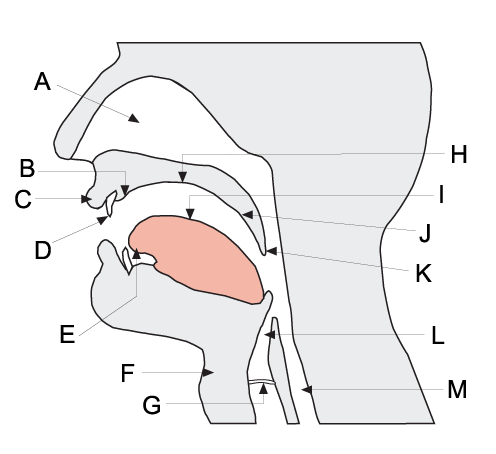
\includegraphics[scale=0.33]{material/04phonoatonomy}
		\end{figure}
	\end{minipage}
	\hfill
	\begin{minipage}{0.4\textwidth}
		
		(\visible<2->{\alertred{G}}) Stimmritze (glottal)\\
		(\visible<3->{\alertred{F}}) Kehlkopf (laryngal)\\
		(\visible<4->{\alertred{B}}) Zahndamm (alveolar)\\
		(\visible<5->{\alertred{A}}) Nasenraum (nasal)\\
		(\visible<6->{\alertred{H}}) harter Gaumen (palatal)\\
		(\visible<7->{\alertred{D}}) Zähne (dental)\\
		(\visible<8->{\alertred{J}}) weicher Gaumen (velar)\\
		(\visible<9->{\alertred{I}}) Zungenrücken (dorsal)\\
		(\visible<10->{\alertred{K}}) Halszäpfchen (uvular)\\
		(\visible<11->{\alertred{C}}) Lippen (labial)\\
		(\visible<12->{\alertred{E}}) Zungenspitze (apikal)
	\end{minipage}
	
\end{itemize}
\end{frame}


%%%%%%%%%%%%%%%%%%%%%%%%%%%%%%%%
\begin{frame}{Hausaufgabe -- Lösung}
\begin{itemize}
	\item[2.] Welcher Laut passt jeweils nicht in die folgenden Reihen?\\Begründen Sie Ihre Entscheidungen.
	
\begin{exe}
	\exr{ex:03aHA2}
\settowidth\jamwidth{XXXXXXXXXXXXXXXXXXXXXXXt}
	\begin{xlist}
		\ex \textipa{[b]}, \textipa{[z]}, \textipa{[a]}, \textipa{[g]}, \textipa{[v]}, \textipa{[p]}, \textipa{[u]} \loesung{2}{\textipa{[p]} (nicht sth., sondern stl.)}
		\ex \textipa{[t]}, \textipa{[s]}, \textipa{[n]}, \textipa{[\c{c}]}, \textipa{[l]}, \textipa{[d]}, \textipa{[r]} \loesung{3}{\textipa{[ç]} (nicht alveolar, sondern palatal)}
		\ex \textipa{[f]}, \textipa{[s]}, \textipa{[x]}, \textipa{[h]}, \textipa{[r]}, \textipa{[z]}
		\loesung{4}{\textipa{[r]} (kein Frikativ, sondern Vibrant)}
		\ex \textipa{[N]}, \textipa{[m]}, \textipa{[k]}, \textipa{[g]}
		\loesung{5}{\textipa{[k]} (nicht sth., sondern stl.)}\loesung{6}{oder: \textipa{[m]} (nicht velar, sondern labial)}
		\ex \textipa{[m]}, \textipa{[b]}, \textipa{[N]}, \textipa{[p]}
		\loesung{7}{\textipa{[N]} (nicht labial, sondern velar)} \loesung{8}{oder: \textipa{[p]} (nicht sth., sondern stl.)}
	\end{xlist}
\end{exe}
	
\end{itemize}
\end{frame}


%%%%%%%%%%%%%%%%%%%%%%%%%%%%%%%%
\begin{frame}{Hausaufgabe -- Lösung}
\begin{itemize}
	\item[3.] Geben Sie die \textbf{phonologische Repräsentation} der folgenden Wörter und \textbf{verschiedene phonetische Realisierungen} (\zB im Paradigma) an und \textbf{erläutern} Sie anschließend den \textbf{Unterschied} zwischen letzteren.
	
\begin{exe}
	\exr{ex:03aHA3}
	\settowidth\jamwidth{XXXXXXXXXXXXXXXXXXXXXXXXXXXXXXXXXXXXXXt}
	\begin{xlist}
		\ex Dieb
		\loesung{2}{\textipa{/di:b/}: \textipa{[di:p], [di:.bə]} -- Auslautverhärtung des \textipa{/b/} in der Koda}
		\ex König
		\loesung{3}{\textipa{/k\o :nıg/}: \textipa{[k\super h\o:.nıç], [k\super h\o:.nı.gə]} --} \loesung{3}{Spirantisierung des \textipa{/g/} in der Koda}
		\ex eng
		\loesung{4}{\textipa{/εng/}: \textipa{[PεN]}, (gegebenenfalls (dialektal) \textipa{[PENk]} -- g-Elision)}
	\end{xlist}
\end{exe}

\end{itemize}

\end{frame}


%%%%%%%%%%%%%%%%%%%%%%%%%%%%%%%%%
\begin{frame}{Hausaufgabe -- Lösung}

\begin{itemize}
	\item[4.] Bestimmen Sie, ob es sich bei den folgenden Lautkombinationen um Affrikaten handeln kann. Begründen Sie Ihre Entscheidungen.

\begin{exe}	
	\exr{ex:03aHA4}
\settowidth\jamwidth{XXXXXXXXXXXXXXXXXXXXXXXXXXXXXXXXXXXXXXX}
	\begin{xlist}
		\ex \textipa{[kl]} \loesung{2}{keine Affrikate (Zweitglied ist kein Frikativ)}
		\ex \textipa{[pf]} \loesung{3}{Affrikate (Verbindung aus Plosiv und homorganem Frikativ)}
		\ex \textipa{[st]} \loesung{4}{keine Affrikate (Plosiv ist Zweitglied)}
		\ex \textipa{[tr]} \loesung{5}{keine Affrikate (Zweitglied ist kein Frikativ)}
		\ex \textipa{[ts]} \loesung{6}{Affrikate (Verbindung aus Plosiv und homorganem Frikativ)}
	\end{xlist}
\end{exe}

\end{itemize}

\end{frame}




%% -*- coding:utf-8 -*-

%%%%%%%%%%%%%%%%%%%%%%%%%%%%%%%%%%%%%%%%%%%%%%%%%%%%%%%%%


\def\insertsectionhead{\refname}
\def\insertsubsectionhead{}

\huberlinjustbarfootline


\ifpdf
\else
\ifxetex
\else
\let\url=\burl
\fi
\fi
\begin{multicols}{2}
{\tiny
%\beamertemplatearticlebibitems

\bibliography{gkbib,bib-abbr,biblio}
\bibliographystyle{unified}
}
\end{multicols}





%% \section{Literatur}
%% \begin{frame}[allowframebreaks]
%% \frametitle{Literatur}
%% 	\footnotesize

%% \bibliographystyle{unified}

%% 	%German
%% %	\bibliographystyle{deChicagoMyP}

%% %	%English
%% %	\bibliographystyle{chicago} 

%% 	\bibliography{gkbib,bib-abbr,biblio}
	
%% \end{frame}


%%%%%%%%%%%%%%%%%%%%%%%%%%%%%%%%%%%
\begin{frame}
\textcolor{white}{
\ea\label{ex:03aHA2}
\ex\label{ex:03aHA3}
\ex\label{ex:03aHA4}
\z
}
\end{frame}

\end{document}